\chapter{植物的气体交换与汁液运输}\label{ch:b1:plant-transport}

在离地一百米的红杉树顶，水分正在
被叶片的蒸发从土壤中拉出，向上穿过
一列管径不超过头发丝的死\omterm{def:b1:cell-unit-of-life:cell}{细胞}，张力之大
足以拉断同样截面的钢丝。这里没有泵；水
靠的是使它自身相互黏附的同一种\omterm{def:b1:water-small-molecules:water}{氢键}来牵引。
与此同时，在旁边的第二组管道中，
那些叶片制造的糖正沿相反方向流动，
由叶片自身产生的压力推动。植物的两套
输导系统即\omterm{def:b1:flowering-plant-organization:tissues}{木质部}与\omterm{def:b1:plant-transport:phloem}{韧皮部}，由植物建立的
物理规律驱动，此后便任其运转。本章讲述叶片借以
用水换取二氧化碳的\omterm{def:b1:plant-transport:stoma}{气孔}、托起汁液的内聚–张力机制、
输送汁液的\omterm{def:b1:flowering-plant-organization:tissues}{导管}、
推动糖分移动的\omterm{thm:b1:plant-transport:pressureflow}{压力流}机制，以及饮水与进食之间的
支配全局的权衡。

\section{气孔：闸门}

\begin{definition}[气孔、保卫细胞]\label{def:b1:plant-transport:stoma}
\index{气孔}\index{保卫细胞}
称\emph{气孔}为叶片（或绿色茎）\omterm{def:b1:flowering-plant-organization:tissues}{表皮}上的孔隙，
由两个\emph{保卫\omterm{def:b1:cell-unit-of-life:cell}{细胞}}围成，保卫\omterm{def:b1:cell-unit-of-life:cell}{细胞}呈肾形，其\omterm{def:b1:eukaryotic-cell:plantcell}{细胞壁}
朝向孔隙一侧增厚，其\omterm{def:b1:carbohydrates:polysaccharide}{纤维素}微纤丝
环绕\omterm{def:b1:cell-unit-of-life:cell}{细胞}呈箍状排列。保卫\omterm{def:b1:cell-unit-of-life:cell}{细胞}吸水
膨胀时，箍状结构阻止其横向扩张，迫使其向两侧弯曲
分开，孔隙随之张开；失水时孔隙关闭。叶片
每平方毫米约有数百个气孔，大多位于下表面；
张开时，孔隙面积占叶片面积的百分之一至二，
而叶片几乎全部的气体交换都经由这些孔隙进行。
\end{definition}

\begin{omfigure}
\begin{tikzpicture}
  \node[anchor=south west, inner sep=0] (img) at (0,0)
    {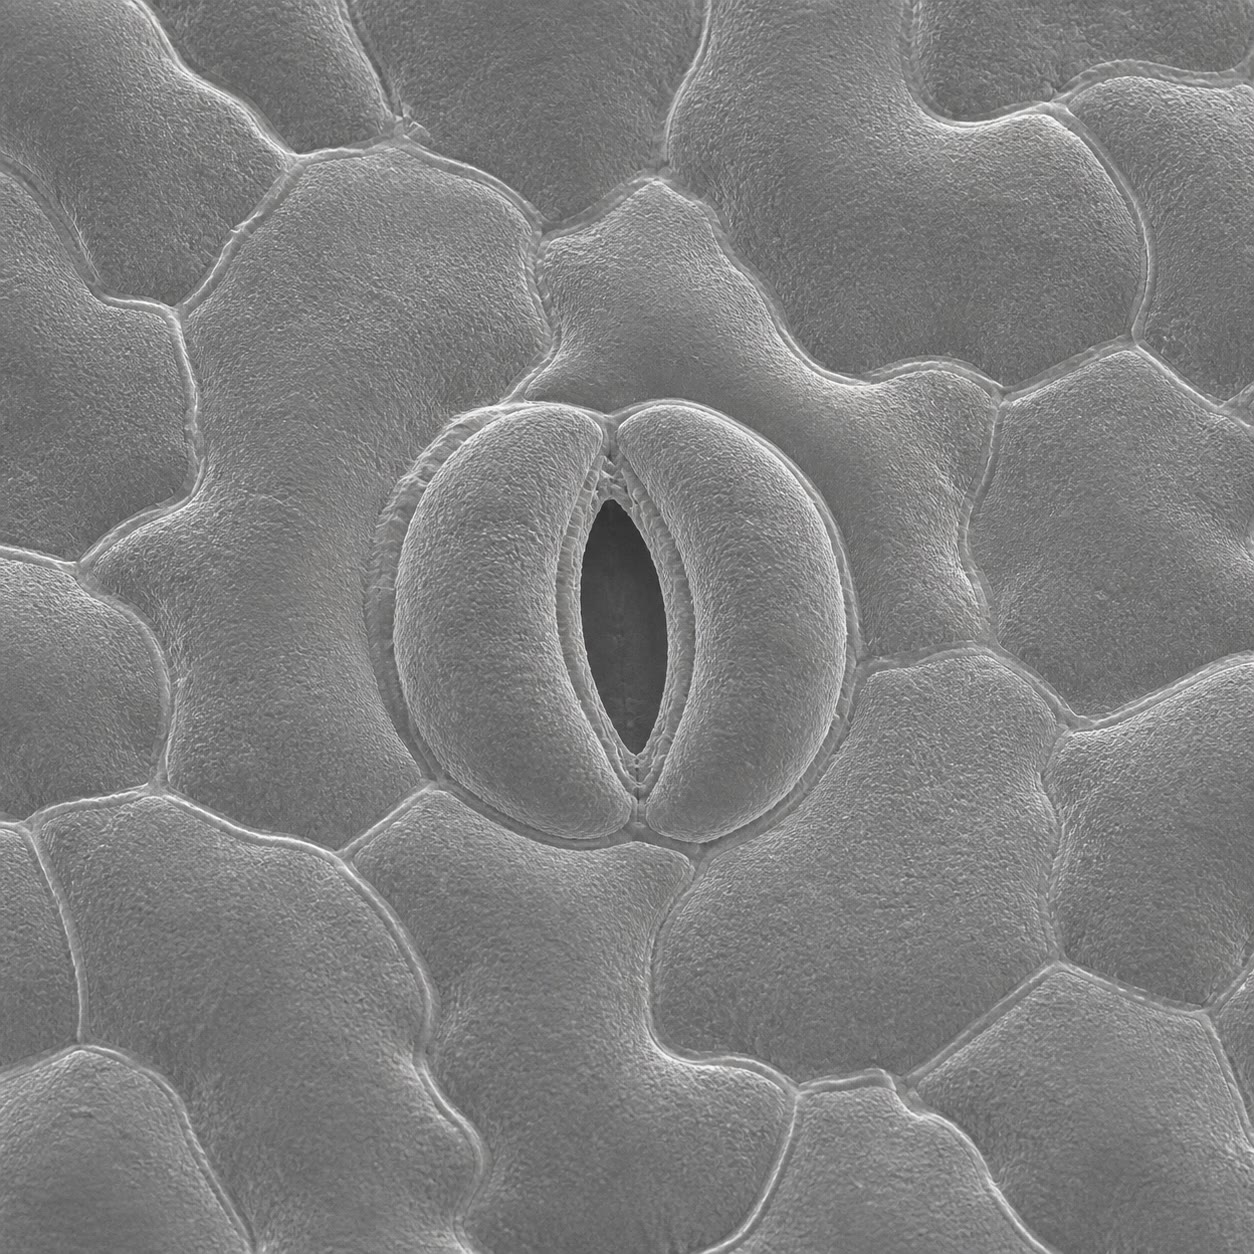
\includegraphics[width=0.4\linewidth]{images/book2/ai/g12-plant-stoma-sem.jpg}};
  \begin{scope}[x={(img.south east)}, y={(img.north west)},
      every node/.style={font=\small}]
    \draw[omDef, thick] (0.50,0.50) -- (0.50,1.08) node[above] {孔隙};
    \draw[omDef, thick] (0.30,0.55) -- (-0.03,0.70) node[left, align=right] {保卫细胞：\\ 增厚的内壁};
    \draw[omDef, thick] (0.80,0.30) -- (1.03,0.20) node[right, align=left] {表皮细胞 \\ 带角质层};
  \end{scope}
\end{tikzpicture}

{\small 从外侧看到的\omterm{def:b1:plant-transport:stoma}{气孔}：孔隙周围为两个\omterm{def:b1:plant-transport:stoma}{保卫细胞}，
嵌于蜡质\omterm{def:b1:flowering-plant-organization:tissues}{表皮}中。\omterm{def:b1:plant-transport:stoma}{保卫细胞}膨胀时，孔隙张开。}
\end{omfigure}

\begin{proposition}[气孔如何张开及何时张开]\label{prop:b1:plant-transport:opening}
\index{脱落酸}
\omterm{def:b1:plant-transport:stoma}{保卫细胞}通过向外泵出质子（见\cref{ch:b1:plant-water-minerals}）来打开孔隙，
这驱动钾离子和氯离子流入，并在\omterm{def:b1:cell-unit-of-life:cell}{细胞}内生成苹果酸；溶质
降低其\omterm{def:b1:membranes-transport:osmosis}{水势}，水分随之从
邻近\omterm{def:b1:cell-unit-of-life:cell}{细胞}中吸水，\omterm{def:b1:eukaryotic-cell:plantcell}{膨压}升高一兆帕。逆转
离子通量的逆转可在数分钟内关闭孔隙。信号有：\emph{光}
（直接照射\omterm{def:b1:plant-transport:stoma}{保卫细胞}的蓝光，以及光合作用开始后胞内
$\mathrm{CO_2}$ 下降）使其张开；\emph{胞内高
$\mathrm{CO_2}$}浓度使其关闭；\emph{水分胁迫}使其关闭，经由
激素\emph{\omterm{prop:b1:plant-transport:opening}{脱落酸}}，由萎蔫的根和叶合成，
它在数分钟内引起\omterm{def:b1:plant-transport:stoma}{保卫细胞}失去离子；干燥的空气
也使其关闭。当碳值得付出水分代价时，叶片开启闸门，
水分稀缺时则关闭——大多数植物按
日节律行事：黎明开启、黄昏关闭，并在
恒定光照下持续数日。
\end{proposition}

\begin{omfigure}
\begin{tikzpicture}
\begin{axis}[
  width=0.88\linewidth, height=6.0cm,
  axis x line=bottom, axis y line=left,
  xmin=0, xmax=24, ymin=0, ymax=1.15,
  xlabel={一日中的时刻 (h)}, ylabel={相对值},
  xlabel style={font=\small, at={(axis description cs:0.5,-0.12)}, anchor=north},
  ylabel style={font=\small},
  tick label style={font=\small}, xtick={0,4,8,12,16,20,24}, ytick={0,0.5,1},
  legend style={font=\small, at={(0.5,-0.24)}, anchor=north, draw=none, legend columns=3, /tikz/every even column/.append style={column sep=0.4cm}},
  clip=false,
]
\addplot[very thick, omExo, smooth] coordinates {(0,0.05) (5,0.05) (6,0.3) (7,0.8) (8,1.0) (11,1.0) (12,0.75) (13,0.5) (14,0.55) (16,0.8) (18,0.6) (19,0.2) (20,0.05) (24,0.05)};
\addlegendentry{气孔开放}
\addplot[very thick, omDef, smooth] coordinates {(0,0) (5,0) (6,0.1) (8,0.5) (10,0.85) (12,1.0) (14,0.9) (16,0.6) (18,0.3) (19,0.1) (20,0) (24,0)};
\addlegendentry{蒸腾作用}
\addplot[very thick, omThm, smooth] coordinates {(0,0.2) (5,0.2) (7,0.3) (9,0.55) (11,0.8) (13,1.0) (15,0.95) (17,0.7) (19,0.4) (21,0.25) (24,0.2)};
\addlegendentry{叶片水势（符号反转）}
\end{axis}
\end{tikzpicture}

{\small 叶片的一个夏日。\omterm{def:b1:plant-transport:stoma}{气孔}黎明时开启，
蒸腾作用随阳光与空气干燥程度上升，同时
叶片\omterm{def:b1:membranes-transport:osmosis}{水势}因水柱承受张力而下降；
正午时分，在干燥空气中，\omterm{def:b1:plant-transport:stoma}{气孔}部分关闭，
叶片\omterm{def:b1:membranes-transport:osmosis}{水势}在午后前略有恢复。}
\end{omfigure}

\section{水分上升：内聚与张力}

\begin{theorem}[内聚–张力机制]\label{thm:b1:plant-transport:cohesiontension}
\index{内聚–张力理论}\index{蒸腾作用}
水在\omterm{def:b1:flowering-plant-organization:tissues}{木质部}中上升，是因为它被从上方\emph{拉动}，而非
从下方推动。叶肉\omterm{def:b1:cell-unit-of-life:cell}{细胞}湿润的\omterm{def:b1:eukaryotic-cell:plantcell}{细胞壁}向气腔
蒸发（\emph{蒸腾作用}）牵引\omterm{def:b1:eukaryotic-cell:plantcell}{细胞壁}细孔中的水，
使之进入弯月面，其表面张力使后方的水
处于张力之下；张力
经由\omterm{def:b1:flowering-plant-organization:tissues}{木质部}中连续的水柱传递，水柱靠内聚力维系
（即\omterm{def:b1:water-small-molecules:water}{氢键}，见
\cref{ch:b1:water-small-molecules}），向下延伸至茎并深入根部，
并从土壤中提升水分。要使高度为 $h$ 的水柱
抵抗重力需要张力 $\rho g h$——\qty{1}{MPa}，每百米
——再加上克服流动摩擦所需的张力，
大致与之相当；高大树木的水柱处于\qtyrange{-2}{-3}{MPa}，
远低于细管中水的抗拉强度。
\end{theorem}
\begin{proof}[证据]
狄克逊与若利（1894）证明，密封玻璃管中的水
能承受数兆帕的张力而不断裂，并且
一根蒸腾中的带叶枝条，密封接于一根
下端插入水银的水管，将水银提得比大气压所能提的更高。
斯科兰德的\emph{压力室}（1965）直接测量张力：
将切下的叶片连同伸出的叶柄一起密封于室中，
刚好迫使汁液退回切口的气体压力
等于汁液所承受的张力——\qtyrange{0.5}{1}{MPa}，
正午水分充足的作物中为此值，\qtyrange{2}{4}{MPa}则见于沙漠灌木
或高大树木的树冠。树径计显示树干在白天
缩小，因张力挤压\omterm{def:b1:flowering-plant-organization:tissues}{导管}；夜间
膨胀；木材中的温度计显示，汁液在蒸腾
最强时流动最快，夜间则停止。无须任何活\omterm{def:b1:cell-unit-of-life:cell}{细胞}参与：
毒杀或加热杀死的茎仍能输导水分。
\end{proof}

\begin{omfigure}
\begin{tikzpicture}[font=\footnotesize, >=Stealth, line cap=round]
  % leaf at top, stem, root in soil; water potentials
  \draw[thick, omExo!70!black, fill=omExo!25] (0,7.0) .. controls (1.4,7.8) and (2.6,7.6) .. (3.0,7.0) .. controls (2.6,6.4) and (1.4,6.2) .. (0,7.0);
  \node[font=\scriptsize] at (1.5,7.0) {叶，$\Psi = \qty{-1.5}{MPa}$};
  \draw[line width=6pt, omDef!35] (1.5,6.3) -- (1.5,1.6);
  \draw[very thick, omDef!70!black] (1.38,6.3) -- (1.38,1.6) (1.62,6.3) -- (1.62,1.6);
  \node[font=\scriptsize, anchor=west, align=left] at (1.75,4.0) {木质部：张力下连续的水柱 \\ 在中部高度处，$\Psi = \qty{-1.0}{MPa}$};
  \fill[pattern=north east lines, pattern color=omProp!60] (-1.0,0) rectangle (4.0,1.6);
  \draw[thick, omDef!60!black] (1.5,1.6) -- (1.5,0.6) (1.5,1.3) -- (0.6,0.4) (1.5,1.0) -- (2.4,0.3);
  \node[font=\scriptsize, anchor=west] at (2.7,1.1) {根，$\Psi = \qty{-0.5}{MPa}$};
  \node[font=\scriptsize, anchor=west] at (2.7,0.5) {土壤，$\Psi = \qty{-0.2}{MPa}$};
  % evaporation arrows out of leaf
  \foreach \x in {0.6,1.5,2.4} { \draw[->, thick, omThm] (\x,7.55) -- (\x,8.3); }
  \node[anchor=south, omThm] at (1.5,8.35) {蒸腾至空气中，$\Psi = \qty{-95}{MPa}$};
  % upward flow arrow
  \draw[->, very thick, omDef!70!black] (-0.6,1.8) -- (-0.6,6.4) node[midway, left, align=right] {汁液向上 \\ 拉动};
  \node[anchor=north, align=center, gray] at (1.5,-0.3) {$\Psi$ 从土壤到空气逐级下降：梯度由顶部的蒸发决定，\\ 水的内聚力将拉力传递至根部};
\end{tikzpicture}

{\small 内聚–张力。叶片处的蒸发降低了该处的\omterm{def:b1:membranes-transport:osmosis}{水势}。
张力沿\omterm{def:b1:flowering-plant-organization:tissues}{木质部}中连续不断的水柱向下传递，
并从土壤中吸取水分。树木本身并不做功，
做功的是太阳。}
\end{omfigure}

\begin{definition}[木质部导管，空穴化]\label{def:b1:plant-transport:xylem}
\index{木质部导管}\index{空穴化}
水分经\omterm{def:b1:flowering-plant-organization:tissues}{木质部}的\emph{\omterm{def:b1:flowering-plant-organization:tissues}{管胞}}和\emph{\omterm{def:b1:flowering-plant-organization:tissues}{导管}}输送，
（见\cref{ch:b1:flowering-plant-organization}）：死\omterm{def:b1:cell-unit-of-life:cell}{细胞}，内容物已排空，
\omterm{def:b1:eukaryotic-cell:plantcell}{细胞壁}木质化，并以环纹和螺纹加厚，
以防在内部张力下塌陷，首尾相接，
通过穿孔（\omterm{def:b1:flowering-plant-organization:tissues}{导管}）或侧壁上的纹孔（\omterm{def:b1:flowering-plant-organization:tissues}{管胞}）相连。
\omterm{def:b1:flowering-plant-organization:tissues}{导管}直径可达\qtyrange{20}{300}{\micro m}，
长可达厘米至米，宽管输导的水分多得多（流量
随管半径的四次方增加），但也更
易发生\emph{空穴化}——即张力下的水中突然形成一个
气泡，使\omterm{def:b1:flowering-plant-organization:tissues}{导管}排空并
退出运行。\omterm{def:b1:flowering-plant-organization:tissues}{导管}之间的纹孔可阻止气泡蔓延；凝固
与干旱均会引起空穴化，树木\omterm{def:b1:flowering-plant-organization:tissues}{导管}部分
借\omterm{prop:b1:plant-water-minerals:rootpressure}{根压}于春季重新充水，或每年由新生木材替换。
\end{definition}

\begin{omfigure}
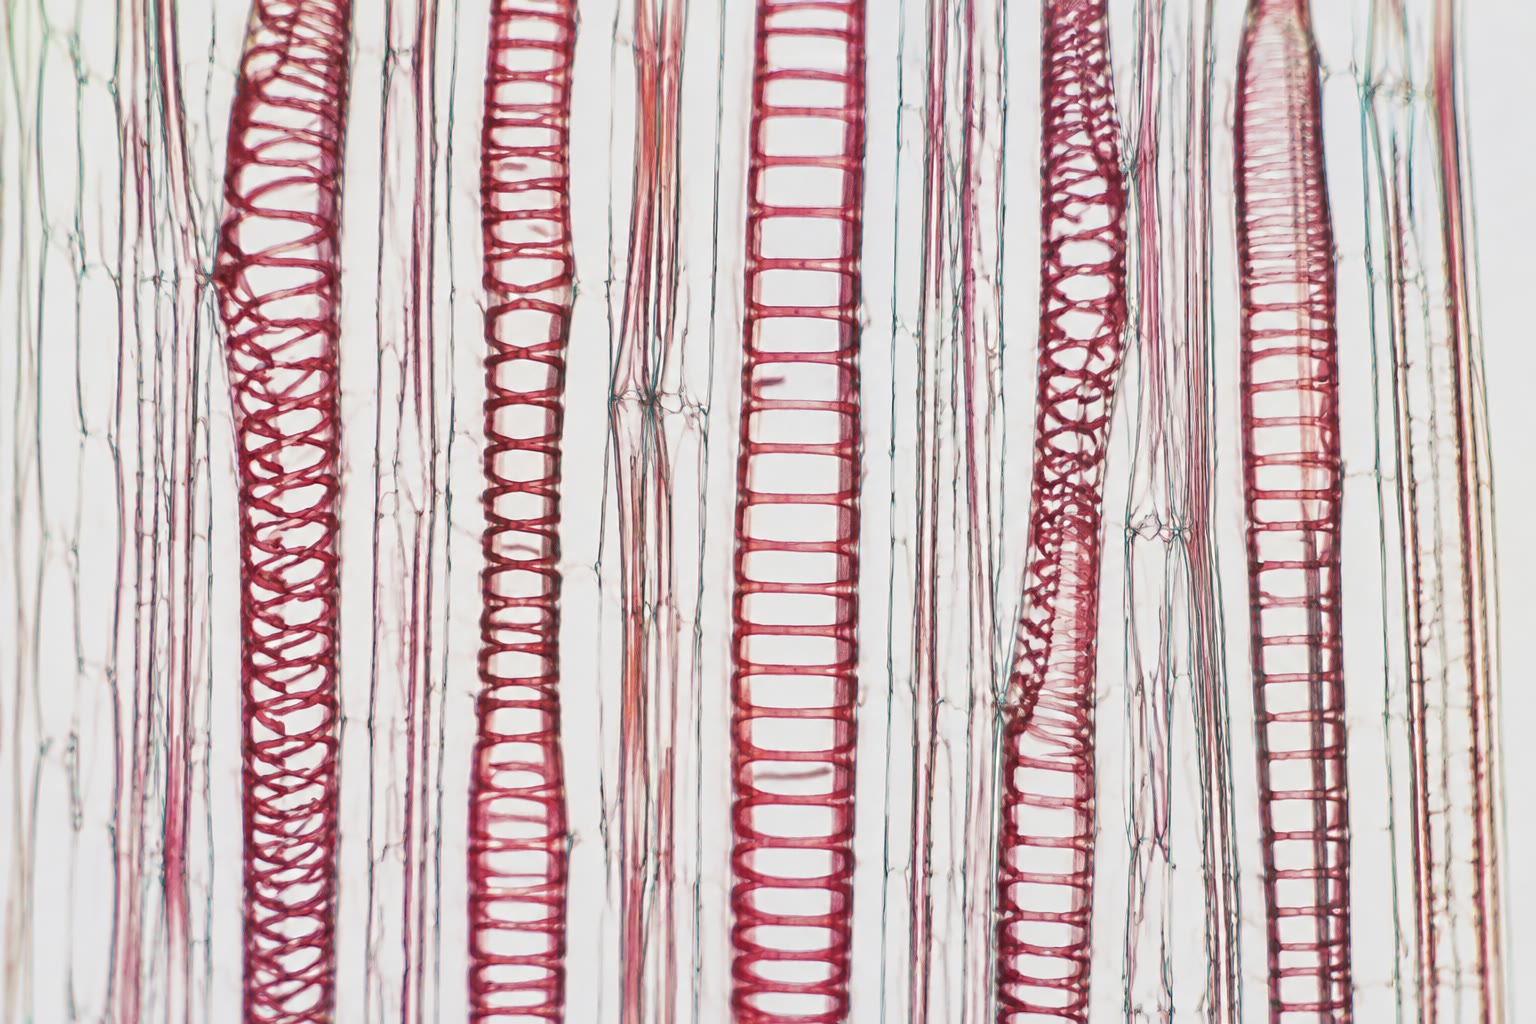
\includegraphics[width=0.52\linewidth]{images/book3/ai/b3-24-xylem-vessels.jpg}

{\small \omterm{def:b1:flowering-plant-organization:tissues}{导管}纵切面：中空的管状结构，其
管壁以木质素构成的环纹和螺纹加固，以抵抗
所输送汁液中的张力。}
\end{omfigure}

\begin{omfigure}
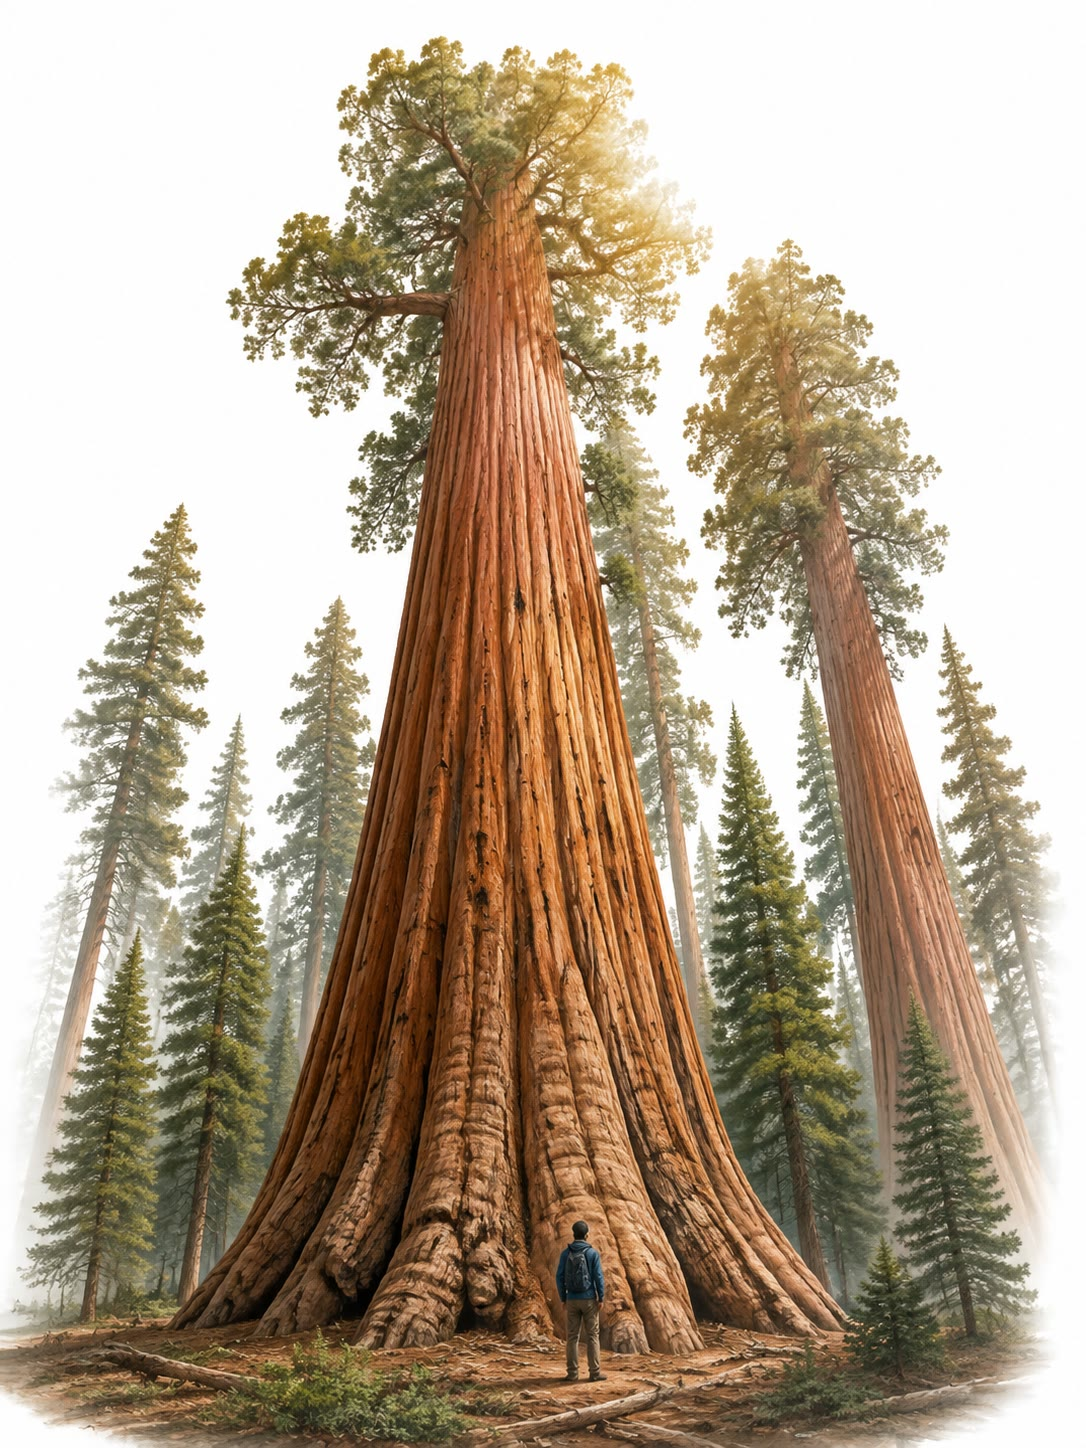
\includegraphics[width=0.36\linewidth]{images/book3/ai/b3-24-sequoia.jpg}

{\small 巨杉。汁液可升至百米高的树冠，
由叶片蒸发牵引，经由水柱
传递，水柱承受两兆帕或更高的张力。}
\end{omfigure}

\begin{example}[树梢]\label{ex:b1:plant-transport:top}
在\qty{100}{m}处，仅水柱自重就需要\qty{1}{MPa}
的张力；白天\omterm{def:b1:flowering-plant-organization:tissues}{导管}中的摩擦力又增加同样多，因此
树冠处的\omterm{def:b1:flowering-plant-organization:tissues}{木质部}\omterm{def:b1:membranes-transport:osmosis}{水势}接近\qty{-2}{MPa}，叶片\omterm{def:b1:cell-unit-of-life:cell}{细胞}要从中吸水，
其\omterm{def:b1:membranes-transport:osmosis}{水势}必须比这更低：其\omterm{def:b1:plant-transport:stoma}{气孔}须在一天中较早关闭，
且其光合作用比低处枝条慢，
树梢的叶片又小又厚。最高的树木约达\qty{120}{m}，
其高度很可能由此决定：超过这一高度，叶片
便无法在干燥的午后维持张力而不发生\omterm{def:b1:plant-transport:xylem}{空穴化}。
\end{example}

\section{糖的运输：压力流}

\begin{definition}[韧皮部、筛管、源与库]\label{def:b1:plant-transport:phloem}
\index{韧皮部}\index{筛管}\index{源}\index{库}
糖经\emph{韧皮部}中的\emph{筛管}运输：一列列
活\omterm{def:b1:cell-unit-of-life:cell}{细胞}，已失去\omterm{def:b1:eukaryotic-cell:nucleus}{细胞核}和大部分\omterm{def:b1:eukaryotic-cell:organelle}{细胞器}，却仍保有
其膜，首尾经有孔的\emph{筛板}相连，
每个\omterm{def:b1:cell-unit-of-life:cell}{细胞}由一个\emph{伴胞}照料，伴胞为其供应
\omterm{def:b1:proteins:peptide}{蛋白质}和 \omterm{def:b1:water-small-molecules:atp}{ATP}。汁液中蔗糖占\qtyrange{10}{30}{\%}，另含\omterm{def:b1:proteins:aminoacid}{氨基
酸}、离子和信号分子，汁液从
\emph{源}——进行光合作用的叶片，或正被排空的贮藏\omterm{def:b1:mammal-organization:organ}{器官}，
流向\emph{库}——生长的顶端、根、果实、种子，
正被充实的贮藏\omterm{def:b1:mammal-organization:organ}{器官}——流速为\qtyrange{0.5}{1}{m/h}，
可朝任意方向流动，不同筛管中的流向也可各异。
\end{definition}

\begin{theorem}[压力流]\label{thm:b1:plant-transport:pressureflow}
\index{压力流机制}
\omterm{def:b1:plant-transport:phloem}{韧皮部}汁液以整体流动的方式移动，其驱动力为
源与库之间的静水压差（明希，1930）。在源处，
伴胞将蔗糖逆梯度\emph{装载}入\omterm{def:b1:plant-transport:phloem}{筛管}，
（经由质子同向运输，取自\omterm{def:b1:plant-water-minerals:pathways}{质外体}，或经
\omterm{def:b1:eukaryotic-cell:plantcell}{胞间连丝}）进入；\omterm{def:b1:plant-transport:phloem}{筛管}的\omterm{def:b1:membranes-transport:osmosis}{水势}下降，水分由
邻近的\omterm{def:b1:flowering-plant-organization:tissues}{木质部}进入，\omterm{def:b1:eukaryotic-cell:plantcell}{膨压}升至\qty{1}{MPa}或更高。
在库处，蔗糖被\emph{卸载}并被消耗或贮存，
\omterm{def:b1:membranes-transport:osmosis}{水势}升高，水分流出，\omterm{def:b1:eukaryotic-cell:plantcell}{膨压}低。两者之间，
汁液沿压力梯度向下，经过筛板，
同时携带其中溶解的各种物质。植物仅在
两端耗能；流动本身是被动的。
\end{theorem}
\begin{proof}[证据]
一只取食茎部的蚜虫将口针插入一根\omterm{def:b1:plant-transport:phloem}{筛管}；
剪去蚜虫后，留在原位的口针便在该\omterm{def:b1:plant-transport:phloem}{筛管}自身压力下
连续数小时渗出汁液——纯净的\omterm{def:b1:plant-transport:phloem}{韧皮部}汁液，其蔗糖浓度
与流速均可测定，其压力
用口针上的压力计测得，在源附近约为\qty{1}{MPa}，
靠近库处则更低。被标记的 $\mathrm{^{14}CO_2}$ 喂入叶片后，
数分钟内即出现在茎的\omterm{def:b1:plant-transport:phloem}{韧皮部}中，其移动速度
与口针流量所预测的一致；冷却一段茎，
这会减慢活\omterm{def:b1:cell-unit-of-life:cell}{细胞}，却几乎不影响压力驱动的流动，
运输仅稍有减慢；毒害源叶的装载，
则使运输停止。
\end{proof}

\begin{omfigure}
\begin{tikzpicture}[font=\footnotesize, >=Stealth, line cap=round]
  % xylem and phloem tubes side by side
  \draw[line width=8pt, omDef!25] (1.0,0.3) -- (1.0,5.7); \node[anchor=south, omDef!70!black] at (1.0,5.8) {木质部};
  \draw[line width=8pt, omExo!25] (3.6,0.3) -- (3.6,5.7); \node[anchor=south, omExo!70!black] at (3.6,5.8) {韧皮部（筛管）};
  % source at top
  \node[draw, thick, rounded corners=4pt, fill=omExo!15, align=center, minimum width=26mm] (src) at (7.2,5.0) {源：叶 \\ 装载蔗糖};
  \node[draw, thick, rounded corners=4pt, fill=omProp!15, align=center, minimum width=26mm] (snk) at (7.2,1.0) {库：根、果实 \\ 卸载蔗糖};
  \draw[->, thick, omExo!70!black] (src.west) -- (3.9,5.0) node[midway, above, font=\scriptsize] {蔗糖流入};
  \draw[->, thick, omProp!80!black] (3.3,1.0) -- (snk.west) node[midway, above, font=\scriptsize] {蔗糖流出};
  % water in from xylem at top, out to xylem at bottom
  \draw[->, thick, omDef!70!black] (1.3,4.6) -- (3.3,4.6) node[midway, below, font=\scriptsize] {水分跟随};
  \draw[->, thick, omDef!70!black] (3.3,1.5) -- (1.3,1.5) node[midway, below, font=\scriptsize] {水分返回};
  % flow arrows
  \draw[->, very thick, omExo!70!black] (3.6,4.2) -- (3.6,2.0) node[midway, right, align=left, font=\scriptsize] {沿压强梯度的 \\ 整体流动};
  \draw[->, very thick, omDef!70!black] (1.0,2.0) -- (1.0,4.2) node[midway, left, align=right, font=\scriptsize] {蒸腾流 \\ （张力）};
  \node[anchor=west, font=\scriptsize] at (3.9,5.5) {$\Psi_p \approx \qty{+1.0}{MPa}$};
  \node[anchor=west, font=\scriptsize] at (3.9,0.5) {$\Psi_p \approx \qty{+0.3}{MPa}$};
\end{tikzpicture}

{\small \omterm{thm:b1:plant-transport:pressureflow}{压力流}。源处装载蔗糖，从\omterm{def:b1:flowering-plant-organization:tissues}{木质部}吸入水分，并使压强升高；
库处卸载蔗糖，水分随之流出，压强降低；汁液在二者之间流动，
水分则
经\omterm{def:b1:flowering-plant-organization:tissues}{木质部}返回。}
\end{omfigure}

\begin{omfigure}
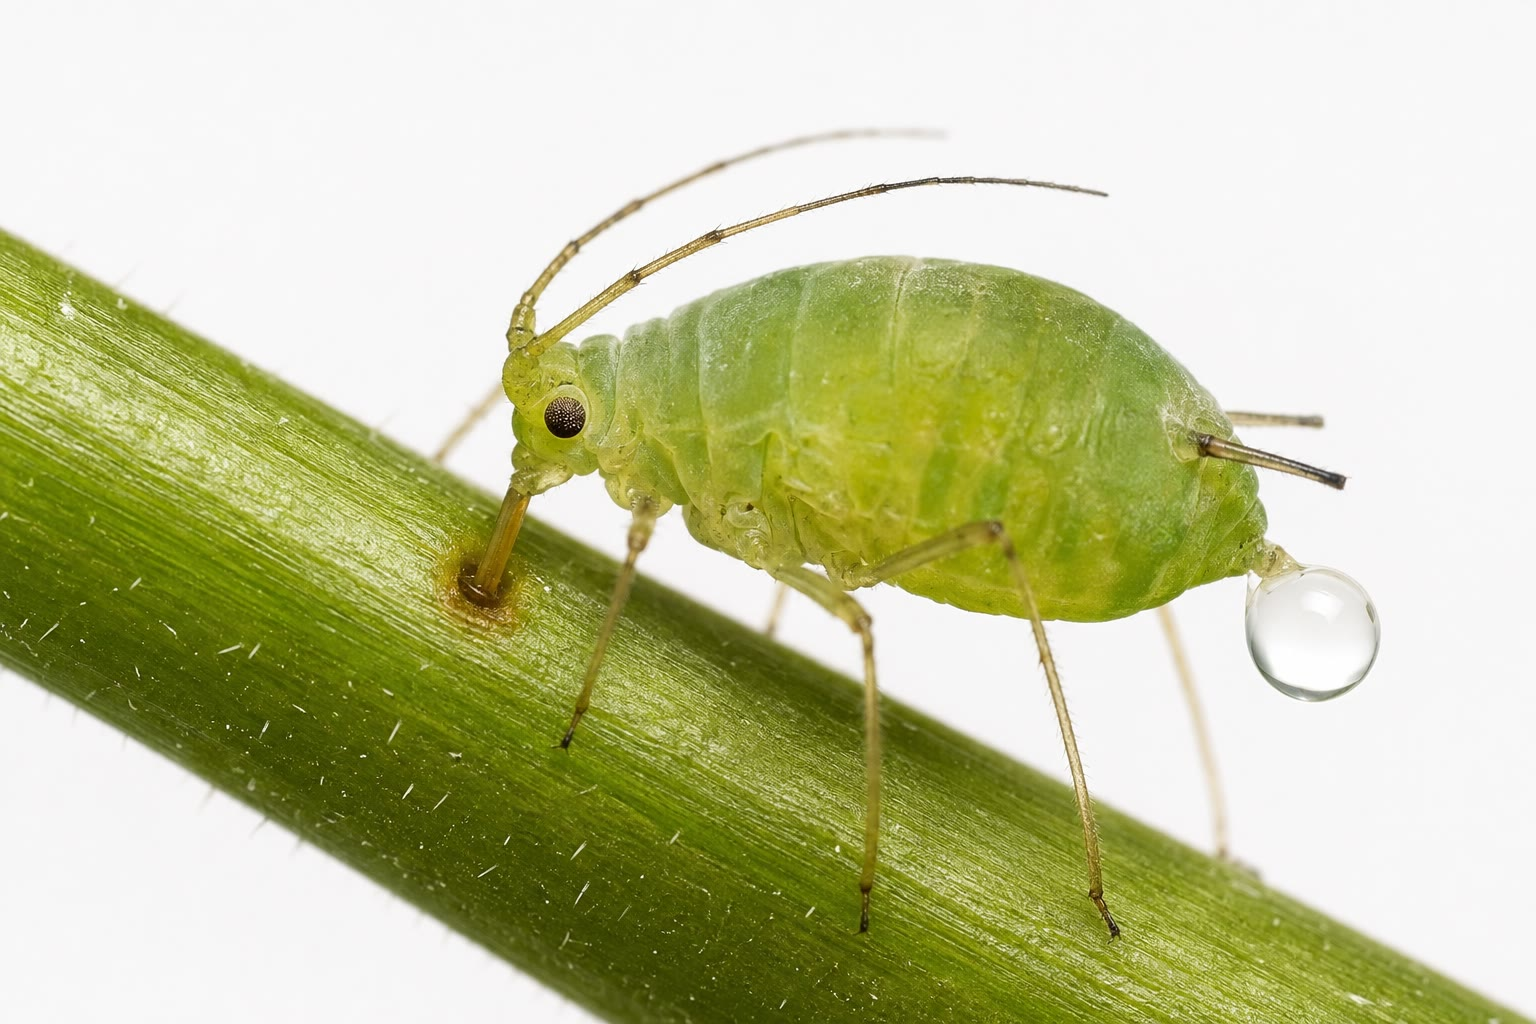
\includegraphics[width=0.5\linewidth]{images/book3/ai/b3-24-aphid-feeding.jpg}

{\small 蚜虫取食茎干：其口针细于毛发，
插入一根\omterm{def:b1:plant-transport:phloem}{筛管}之中，\omterm{def:b1:plant-transport:phloem}{韧皮部}的压强将汁液压入昆虫体内——
量之多，以至于多余的部分以蜜露的形式排出体外。剪去蚜虫后，
口针便成为植物生理学家的“水龙头”。}
\end{omfigure}

\begin{method}[读取韧皮部运输实验]\label{met:b1:plant-transport:translocation}
\begin{enumerate}
  \item 用标记的 $\mathrm{CO_2}$ 喂养一片叶；在茎的上方与下方间隔取样：
        标记物位置随时间的变化
        给出流动的方向与速度。
  \item 环剥茎干（去除一圈树皮，树皮中含有\omterm{def:b1:plant-transport:phloem}{韧皮部}，而保留\omterm{def:b1:flowering-plant-organization:tissues}{木质部}）：
        糖分在环割处上方积累，下方的根则因缺糖而饥饿——
        运送糖分的是\omterm{def:b1:plant-transport:phloem}{韧皮部}而非\omterm{def:b1:flowering-plant-organization:tissues}{木质部}；
        树在一个季节内死亡。
  \item 从两个高度的被切断的蚜虫口针处收集汁液：
        二者之间蔗糖浓度与压强的下降，
        即驱动流动的梯度。
  \item 改变库：去除果实，标记物则转向根；
        遮蔽叶片，它本身便成为库。
        流动的格局即是需求的格局。
\end{enumerate}
\end{method}

\begin{example}[一株马铃薯的两个季节]\label{ex:b1:plant-transport:potato}
夏季，叶片是源，地下的块茎是库：蔗糖向下流动，
被卸载，转化为\omterm{def:b1:carbohydrates:polysaccharide}{淀粉}，块茎随之膨大。
春季，块茎发芽：其中的\omterm{def:b1:carbohydrates:polysaccharide}{淀粉}重新转化为蔗糖，
装入\omterm{def:b1:plant-transport:phloem}{韧皮部}，并向上流向生长中的芽——
同一根管道，流向却相反，因为源与库
已经互换了位置。
\end{example}

\section{权衡}

\begin{proposition}[水分利用效率]\label{prop:b1:plant-transport:wue}
\index{水分利用效率}
任何允许二氧化碳进入的\omterm{def:b1:plant-transport:stoma}{气孔}都会散失水分，二者的交换却并不对等：
叶内部充满饱和水汽，而外部空气干燥，
外部 $\mathrm{CO_2}$ 为 \qty{0.04}{\%}，内部更低，
因此水分向外的梯度
是二氧化碳向内梯度的数百倍。C3 植物每固定一个
$\mathrm{CO_2}$ 分子，损失 \qtyrange{200}{500}{} 个水分子；C4 叶片
富集 $\mathrm{CO_2}$ 且\omterm{def:b1:plant-transport:stoma}{气孔}较窄，损失 \qtyrange{100}{200}{} 个；CAM 植物
仅在夜间开放\omterm{def:b1:plant-transport:stoma}{气孔}，损失 \qtyrange{20}{50}{} 个
（见\cref{ch:b1:photosynthesis}）。
\emph{\omterm{prop:b1:plant-transport:wue}{水分利用效率}}是单位失水所获得的碳量，其提高——
通过午间关闭\omterm{def:b1:plant-transport:stoma}{气孔}、凹陷的\omterm{def:b1:plant-transport:stoma}{气孔}与厚\omterm{def:b1:flowering-plant-organization:tissues}{角质层}，
以及 C4 与 CAM 途径——
正是植物在干燥大气中达成这笔交易的一方面。
\end{proposition}

\begin{example}[数字中的交易]\label{ex:b1:plant-transport:bargain}
一株玉米每天蒸腾一升半的水，固定约
\qty{10}{g} 二氧化碳：\qty{80}{mol} 水换取
\qty{0.23}{mol} 的 $\mathrm{CO_2}$，比例为三百五十比一。一块小麦田
在一个季节内每公顷蒸腾五百吨水，
以产出八吨谷物；水是碳的代价，
而在世界上大多数农田中，正是这一代价限制了
收成。
\end{example}

\section{练习}

\begin{exercise}[$\star$]\label{exo:b1:plant-transport:1}
解释\omterm{def:b1:plant-transport:stoma}{保卫细胞}的形状与\omterm{def:b1:eukaryotic-cell:plantcell}{细胞壁}如何将\omterm{def:b1:eukaryotic-cell:plantcell}{膨压}的升高
转化为开放的\omterm{def:b1:plant-transport:stoma}{气孔}。
\end{exercise}

\begin{exercise}[$\star$]\label{exo:b1:plant-transport:2}
用三句话陈述内聚–张力机制：力从何处产生，
由什么传递，在根部起什么作用。
\end{exercise}

\begin{exercise}[$\star$]\label{exo:b1:plant-transport:3}
由日变化图，蒸腾作用在何时最强，
叶片\omterm{def:b1:membranes-transport:osmosis}{水势}何时达到最低，
以及\omterm{def:b1:plant-transport:stoma}{气孔}为何在午间部分关闭？
\end{exercise}

\begin{exercise}[$\star$]\label{exo:b1:plant-transport:4}
定义源与库，并说明在
\omterm{thm:b1:plant-transport:pressureflow}{压力流}机制中各自发生什么。
\end{exercise}

\begin{exercise}[$\star\star$]\label{exo:b1:plant-transport:5}
计算维持一根 \qty{30}{m} 高水柱所需的张力
（$\rho g h$），以及摩擦使其加倍后的总张力。该高度处叶片的\omterm{def:b1:membranes-transport:osmosis}{水势}
至少须为多少？
\end{exercise}

\begin{exercise}[$\star\star$]\label{exo:b1:plant-transport:6}
管道中的流量与 $r^4$ 成正比。比较一根半径为
\qty{100}{\micro m} 的\omterm{def:b1:flowering-plant-organization:tissues}{导管}与总截面积相同的若干根
\qty{10}{\micro m} 的\omterm{def:b1:flowering-plant-organization:tissues}{管胞}中的流量。为何
植物保留的是较窄的那些？
\end{exercise}

\begin{exercise}[$\star\star$]\label{exo:b1:plant-transport:7}
\omterm{def:b1:plant-transport:phloem}{韧皮部}汁液中蔗糖含量为 \qty{20}{\%}（\qty{0.6}{mol/L}），其\omterm{def:b1:membranes-transport:osmosis}{溶质势}约为
\qty{-1.5}{MPa}。与\omterm{def:b1:membranes-transport:osmosis}{水势}为 \qty{-0.5}{MPa} 的\omterm{def:b1:flowering-plant-organization:tissues}{木质部}相邻时，
平衡时\omterm{def:b1:plant-transport:phloem}{筛管}的\omterm{def:b1:eukaryotic-cell:plantcell}{膨压}为多少？在库处，汁液中蔗糖含量为
\qty{5}{\%}（$\Psi_s = \qty{-0.4}{MPa}$），与同一\omterm{def:b1:flowering-plant-organization:tissues}{木质部}相邻时，
其\omterm{def:b1:eukaryotic-cell:plantcell}{膨压}为多少？驱动流动的压强差为多少？
\end{exercise}

\begin{exercise}[$\star\star$]\label{exo:b1:plant-transport:8}
一根蚜虫口针每小时渗出 \qty{1}{\micro L} 汁液，其
蔗糖含量为 \qty{20}{\%}。若\omterm{def:b1:plant-transport:phloem}{筛管}半径为
\qty{10}{\micro m}，计算汁液的流速及
每小时输送的糖量。
\end{exercise}

\begin{exercise}[$\star\star$]\label{exo:b1:plant-transport:9}
解释为何环剥一棵树会使其在一个季节之内死亡，而其叶片
在环剥之后仍能保持数周的绿色。
\end{exercise}

\begin{exercise}[$\star\star\star$]\label{exo:b1:plant-transport:10}
叶片的气腔在 \qty{25}{\celsius} 时饱和（蒸气含量为
\qty{23}{g/m^3}）；外部空气中的蒸气含量为 \qty{9}{g/m^3}。
$\mathrm{CO_2}$ 在外部为 \qty{0.72}{g/m^3}，
在内部为 \qty{0.45}{g/m^3}。两种气体经相同的\omterm{def:b1:plant-transport:stoma}{气孔}扩散，水的扩散
速率是 $\mathrm{CO_2}$ 的 1.6 倍。计算
失去的水与获得的 $\mathrm{CO_2}$ 之比，分别按质量和分子数计。
\end{exercise}

\begin{exercise}[$\star\star\star$]\label{exo:b1:plant-transport:11}
炎热干燥的午后，一根\omterm{def:b1:flowering-plant-organization:tissues}{导管}发生\omterm{def:b1:plant-transport:xylem}{空穴化}。描述水柱
会发生什么变化，相邻\omterm{def:b1:flowering-plant-organization:tissues}{导管}中的张力如何变化，以及
其所供应的叶片会受到何种影响；解释纹孔如何限制损伤，以及植物如何
在夜间或春季恢复。
\end{exercise}

\begin{exercise}[$\star\star\star$]\label{exo:b1:plant-transport:12}
“一棵树是土壤与天空之间的一根灯芯，另有一根
方向相反的糖管。”请用一段话讨论：各系统输送什么，
由何驱动，植物在何处耗能，
以及在何处不耗能。
\end{exercise}

\section{问题：红杉}

\begin{problem}[{周末问题——夏日的一棵百米高树：
树冠处的张力、汁液的流速、所输送的水量、
向下输送的糖量及所固定的碳，最后归结为树冠处木质部的
张力}]
\label{pb:b1:plant-transport:1}
一棵红杉高 \qty{100}{m}，树冠的叶面积为 \qty{2000}{m^2}。
夏日白天，它在 \qty{12}{h} 内蒸腾了 \qty{600}{L} 水，
水分经由横截面积为 \qty{0.5}{m^2} 的边材运输，其中 \qty{20}{\%}
为输导腔。水的参数：$\rho = \qty{1000}{kg/m^3}$，$g =
\qty{9.8}{m/s^2}$，\qty{18}{g/mol}。沿树干的摩擦所消耗的张力
与重力相当。土壤\omterm{def:b1:membranes-transport:osmosis}{水势}为 \qty{-0.1}{MPa}。
树冠每平方米叶片每秒固定 \qty{4}{\micro mol} 的 $\mathrm{CO_2}$，
持续 \qty{12}{h}；蔗糖的摩尔质量为 \qty{342}{g/mol}，含十二个碳；
\omterm{def:b1:plant-transport:phloem}{韧皮部}汁液的蔗糖质量分数为 \qty{15}{\%}
（密度为 \qty{1.06}{g/mL}），流速为 \qty{0.6}{m/h}。

\medskip
\noindent\textbf{第一部分——张力。}
\begin{enumerate}
  \item 计算支撑水柱以抵抗重力所需的
        张力。
  \item 计入摩擦，树冠处\omterm{def:b1:flowering-plant-organization:tissues}{木质部}的张力为多少？
  \item 计算树冠处\omterm{def:b1:flowering-plant-organization:tissues}{木质部}的\omterm{def:b1:membranes-transport:osmosis}{水势}，
        取汁液的 $\Psi_s = 0$。
  \item 树冠处叶\omterm{def:b1:cell-unit-of-life:cell}{细胞}的\omterm{def:b1:membranes-transport:osmosis}{水势}须为多少，
        水才能进入\omterm{def:b1:cell-unit-of-life:cell}{细胞}？若其 $\Psi_s = \qty{-2.5}{MPa}$，则
        \omterm{def:b1:eukaryotic-cell:plantcell}{膨压}为多少？
  \item 与同一棵树上 \qty{10}{m} 高处的叶片比较（$\Psi_s =
        \qty{-1.5}{MPa}$）。
  \item 细管中的水可承受约 \qty{-30}{MPa} 的张力；
        为何树木不能直接长到 \qty{1000}{m} 高？
\end{enumerate}

\medskip
\noindent\textbf{第二部分——流动。}
\begin{enumerate}[resume]
  \item 分别以升每小时和
        立方米每秒计算蒸腾速率。
  \item 计算边材的输导截面积。
  \item 计算汁液的平均流速。
  \item 计算树干输导腔中所含水的质量，
        （树干全长 \qty{100}{m}）。
  \item 以此流速，水分子从根运输至
        树冠需要多长时间？
  \item 计算每平方米叶片每小时的蒸腾量，
        分别以克和每秒毫摩尔表示。
  \item 汁液沿\omterm{def:b1:membranes-transport:osmosis}{水势}梯度向下流动，从土壤处的 \qty{-0.1}{}
        降至树冠处第 3 题所得的值，跨越 \qty{100}{m}。
        该梯度以兆帕每米计为多少？它与仅由重力
        所引起的部分相比如何？
\end{enumerate}

\medskip
\noindent\textbf{第三部分——\omterm{def:b1:carbohydrates:monosaccharide}{糖类}。}
\begin{enumerate}[resume]
  \item 计算树冠每天固定的 $\mathrm{CO_2}$ 量，
        以摩尔表示。
  \item 计算与之对应的蔗糖量，分别以摩尔和
        千克表示。
  \item 一半在树冠中被呼吸消耗，其余
        经\omterm{def:b1:plant-transport:phloem}{韧皮部}向下运输。计算每天运输的蔗糖质量，以及
        携带它的汁液的质量。
  \item 计算汁液的体积；若流速为 \qty{0.6}{m/h}，
        求在 \qty{24}{h} 内输送该体积汁液所需的\omterm{def:b1:plant-transport:phloem}{筛管}横截面积。
  \item 计算蔗糖从树冠运输到根部所需的时间。
  \item 计算水分利用比，即每固定一摩尔
        $\mathrm{CO_2}$ 所蒸腾的水的摩尔数。
\end{enumerate}

\medskip
\noindent\textbf{第四部分——权衡。}
\begin{enumerate}[resume]
  \item 树冠处\omterm{def:b1:plant-transport:phloem}{韧皮部}汁液的\omterm{def:b1:membranes-transport:osmosis}{水势}，已知
        $\Psi_s = \qty{-1.2}{MPa}$，\omterm{def:b1:eukaryotic-cell:plantcell}{膨压}为 \qty{1.0}{MPa}，计算其值，
        并与该处\omterm{def:b1:flowering-plant-organization:tissues}{木质部}的\omterm{def:b1:membranes-transport:osmosis}{水势}相比较。两者之间水分向
        哪个方向移动？这与装载是否一致？
  \item 在根部，\omterm{def:b1:plant-transport:phloem}{韧皮部}汁液的蔗糖含量为 \qty{5}{\%}（$\Psi_s =
        \qty{-0.4}{MPa}$），\omterm{def:b1:flowering-plant-organization:tissues}{木质部}的\omterm{def:b1:membranes-transport:osmosis}{水势}为 \qty{-0.3}{MPa}。
        \omterm{def:b1:eukaryotic-cell:plantcell}{膨压}为多少时，\omterm{def:b1:plant-transport:phloem}{韧皮部}的 $\Psi$ 与\omterm{def:b1:flowering-plant-organization:tissues}{木质部}的相等？
        树冠与根部之间的压强差为多少时才能驱动汁液流动？
  \item 中午时\omterm{def:b1:plant-transport:stoma}{气孔}关闭，蒸腾量减半。
        重新计算摩擦张力和树冠\omterm{def:b1:flowering-plant-organization:tissues}{木质部}的\omterm{def:b1:membranes-transport:osmosis}{水势}。
        树木获得了什么，又失去了什么？
  \item 在干旱年份，土壤\omterm{def:b1:membranes-transport:osmosis}{水势}降至 \qty{-1.0}{MPa}，
        在蒸腾量完全的情况下，重新计算树冠的\omterm{def:b1:membranes-transport:osmosis}{水势}。树冠叶片
        （$\Psi_s = \qty{-2.5}{MPa}$）能否保持任何\omterm{def:b1:eukaryotic-cell:plantcell}{膨压}？树木
        必须采取什么措施？
  \item 解释为什么最高的叶片最小且最厚。
  \item 给出结论：夏日某天，一棵 \qty{100}{m} 高的树的树冠处的
        \omterm{def:b1:flowering-plant-organization:tissues}{木质部}张力，
        以及与之对应的汁液流速。
\end{enumerate}
\end{problem}
